\documentclass{beamer}
\usetheme[faculty=econ]{fibeamer}
\usepackage[utf8]{inputenc}
\usepackage[T1]{fontenc}
\usepackage[french]{babel}
\usepackage{ulem}
\usepackage{xcolor}

\usepackage{xcolor}

\definecolor{mypink1}{rgb}{0.858, 0.188, 0.478}
\definecolor{mypink2}{RGB}{219, 48, 122}
\definecolor{mypink3}{cmyk}{0, 0.7808, 0.4429, 0.1412}
\definecolor{mygray}{gray}{0.6}


\colorlet{Mycolor1}{green!10!orange!90!}
\definecolor{Mycolor2}{HTML}{00F9DE}

\lstdefinestyle{C}
{
  language=C,
  escapechar=@, % include LaTeX code between `@' characters
  keepspaces,   % needed to preserve spacing with lstinline
  basicstyle=\scriptsize\ttfamily\bfseries,
  commentstyle=\color{green},
  stringstyle=\color{cyan},
  showstringspaces=false,
  keywordstyle=[1]\color{blue},    % instructions
  keywordstyle=[2]\color{magenta}, % directives
  keywordstyle=[3]\color{red},     % registers
}

\newcommand{\mycolumns}[5]{
\begin{columns}[#1]
    \column{#2cm}
    #4
    \column{#3cm}
    #5
\end{columns}
}

\newcommand{\hlrose}[1]{\sethlcolor{rosepale}\hl{#1}}

\title[Arithmétique flottante]{Représentation des données\break{}-- Arithmétique
flottante}
\author[C.~Tibermacine]{\large{Chouki TIBERMACINE}\\
\vspace{1cm}
\small{Chouki.Tibermacine@umontpellier.fr}}
\institute{Polytech Montpellier}
\date{\tiny{IG3 2018-2019}}

\begin{document}

\begin{frame}
\titlepage
\begin{center}

\includegraphics[width=4cm]{figs/polytech.png}
\end{center}
\end{frame}

\begin{frame}
\frametitle{Représentation des nombres réels}

\begin{itemize}
\item Un nombre réel dans le système décimal peut s'écrire :\\
  $$n = d_md_{m-1}...d_1d_0.d_{-1}d_{-2}...d_{-p}$$\\
  
\begin{minipage}[b]{0.6\linewidth} 
	\item La valeur du nombre :
  		$$n=\sum_{i=-p}^{m} d_i~x~10^i $$
\end{minipage}
\begin{minipage}[b]{0.38\linewidth} 
	\centering
	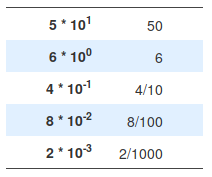
\includegraphics[trim = 0cm 0cm 0cm 0cm, clip,scale=0.3]{figs/positivePower.png} 
\end{minipage}
\item  Exemple : $$23.375=2x10^1+3x10^0+3x10^{-1}+7x10^{-2}+5x10^{-3}=23375/1000$$
\end{itemize}
\end{frame}

\begin{frame}
\frametitle{Nombres réels en binaire}

\begin{itemize}
\item Un nombre réel dans le système binaire peut être écrit :\\
  $$n = b_mb_{m-1}...b_1b_0.b_{-1}b_{-2}...b_{-p}$$\\

\begin{minipage}[b]{0.6\linewidth}
	\item La valeur du nombre :
  		$$n=\sum_{i=-p}^{m} b_i~x~2^i $$
\end{minipage} 
\begin{minipage}[b]{0.38\linewidth} 
	\centering
	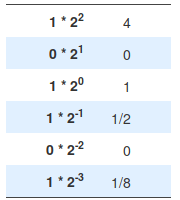
\includegraphics[trim = 0cm 0cm 0cm 0cm, clip,scale=0.25]{figs/negativePower.png} 
\end{minipage}

\item  Exemple : 
\begin{minipage}[b]{0.98\linewidth} 
	\centering
	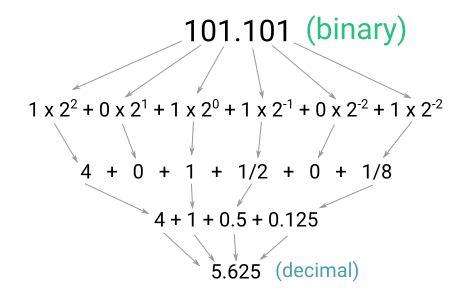
\includegraphics[trim = 0cm 0cm 0cm 0cm, clip,scale=0.25]{figs/floatingValFormation.png} 
\end{minipage}
%$$10.101=1x2^1+0x2^0+1x2^{-1}+0x2^{-2}+1x2^{-3}$$
\end{itemize}
\end{frame}

\begin{frame}
\frametitle{Du décimal au binaire}
\begin{minipage}[b]{0.5\linewidth}
	\begin{itemize}
		\item La multiplication est utilisée
		\item S'il s'agit d'un nombre entier (> = 1.0), le bit est 1
		\item $0.375_{10}$ $\rightarrow$ $?_2$\\
	
	  0.375 x 2 = 0.75 = \colorbox{pink}{0} + 0.75\\
	  0.75 x 2 = 1.5  = \colorbox{pink}{1} + 0.5\\
	  0.5 x 2 = 1.0 = \colorbox{pink}{1} + 0.0\\
	  
	\item $0.375_{10}$ $\rightarrow$ 0.\colorbox{pink}{011}$_2$
	\end{itemize}
\end{minipage}
\begin{minipage}[b]{0.45\linewidth}
	\begin{itemize}
		\item La partie décimale est ensuite utilisée pour le calcul suivant
		\item Une fois que le résultat atteint 1.0, la conversion est terminée
	\end{itemize}
\end{minipage}
\end{frame}

\begin{frame}
\frametitle{Du décimal au binaire}

\begin{minipage}[b]{0.98\linewidth}
	\begin{itemize}
	\item  Il y a beaucoup de nombres qui n'aboutissent pas à un résultat de 1.0
	\item Une fois que le résultat atteint 1.0, la conversion est terminée
	\item Puisqu'il y a $t$ bits possibles pour la mantisse
	\item La conversion se termine dès que $t$ bits sont atteints
	
	\item $0.4_{10}$ $\rightarrow$ $?_2$\\
	
	  0.4 x 2 = 0.8 = \colorbox{pink}{0} + 0.8\\
	  0.8 x 2 = 1.6  = \colorbox{pink}{1} + 0.6\\
	  0.6 x 2 = 1.2 = \colorbox{pink}{1} + 0.2\\
	  0.2 x 2 = 0.4 = \colorbox{pink}{0} + 0.4\\
	  $\Rightarrow$0.4 x 2 = 0.8 = \colorbox{yellow}{0} + 0.8\\
	  
	\item $0.4_{10}$ $\rightarrow$ 0.\colorbox{pink}{0110}\colorbox{yellow}{[0110]}$_2$
	\end{itemize}
\end{minipage}
\end{frame}

\begin{frame}
\frametitle{Du binaire au décimal}

\only<1>{  
  \begin{block}{Quelle est la valeur en décimal des nombres binaires
      suivants ?}
  \begin{itemize}
  \item $0.1_2$ = $?_{10}$
  \item $0.01_2$ = $?_{10}$
  \item $0.11_2$ = $?_{10}$
  \item $0.1001_2$ = $?_{10}$
  \end{itemize}
\end{block}
}
\only<2>{
  \begin{block}{Quelle est la valeur en décimal des nombres binaires suivants ?}
  \begin{itemize}
  \item $0.1_2$ = $0.5_{10}$
  \item $0.01_2$ = $0.25_{10}$
  \item $0.11_2$ = $0.5_{10}$+$0.25_{10}$ = $0.75_{10}$
  \item $0.1001_2$ = $0.5_{10}$+$0.0625_{10}$ = $0.5625_{10}$
  \end{itemize}
\end{block}
}
\end{frame}

\begin{frame}
  \frametitle{Nombres réels en notation scientifique}
  \begin{itemize}
  \item Notation : $\pm m~x~10^n$ ou $\pm m$ E$^e$\\
    où : $\pm$ est le \textbf{signe}, m est la \textbf{mantisse} et $e$
    est l'\textbf{exposant}
  \item 123 400 000 000 000 s'écrit $1.234~x~10^{14}$ ou 1.234E14
  \item 0.000 000 000 000 123 s'écrit $1.23~x~10^{-13}$ ou 1.23E-13
  \end{itemize}
\end{frame}


\begin{frame}
  \frametitle{Nombres réels binaires en virgule flottante
    (équiv. notation scientifique)}
  \begin{itemize}
  \item Dans le cas général, on écrit : $\pm m~x~B^e$\\ où \textcolor{Mycolor1}{B est la base}
  \item Dans le système binaire : $\pm m~x~2^e$\\ où \textcolor{Mycolor2}{$m$ (mantisse)} est
    exprimée \textcolor{Mycolor1}{sous la forme d'un nombre binaire}
  \item En variant \textcolor{Mycolor1}{l'exposant, on fait ``flotter'' la virgule}
  \item Avantage : Pour un même nombre de bits donné, \textcolor{Mycolor1}{on peut
    représenter un intervalle de nombres plus important} que les
    représentations des entiers ou à virgule fixe
  \end{itemize}  
\end{frame}

\begin{frame}
  \frametitle{Codage binaire des nombres réels}
  \begin{center}
    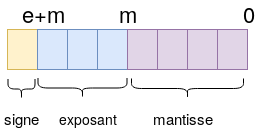
\includegraphics[width=4cm]{img/ieee754.png}
    \hspace{5mm}
    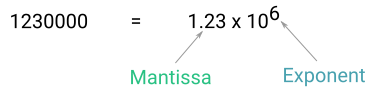
\includegraphics[width=4cm]{figs/minetosa.png}
  \end{center}
  \begin{itemize}
  \item Le codage sur un nombre n (=e+m+1) de bits, fixe, implique un
    nombre fini de valeurs
  \item \textcolor{Mycolor1}{Ceci implique des calculs arrondis (perte de précision) et des erreurs} d'arrondi
  \item Un même nombre peut être représenté de différentes façons :
  $0.110x2^5$ = $110x2^2$ = $0.0110x2^6$
  \end{itemize}  
\end{frame}

\begin{frame}
  \frametitle{Codage binaire des nombres réels -suite-}
  \begin{enumerate}
  	\only<1>{
  \item Convertir séparément les entiers et les décimales
  \item Ajoutez $\times 2^0$ à la fin du nombre binaire (qui ne change pas sa valeur)
  \item Pour \textcolor{Mycolor1}{éviter des représentations différentes d'un même nombre}, la mantisse est normalisée
  \begin{itemize}
  		\item Couramment, un nombre (différent de zéro) avec une mantisse normalisée a la forme	suivante~: $\pm1.bbb...x2^e$\\
    	\item Le chiffre 1 à gauche du point décimal est retiré de la
    représentation pour gagner un bit (il devient implicite)
    \end{itemize}
 \item Avec la notation normalisée (mantisse : \colorbox{red}{1}.bbb x $2^e$), \textcolor{Mycolor1}{omettez 1 tout à gauche et remplissez avec des zéros à droite}
	}
\only<2>{
 \item Représenter l'exposant avec un décalage (``Biais'')
 \item Biais = $2^{|e|-1}-1$ (|e| : taille de l'exposant)
 \item Pour un exposant sur |e| bits : au lieu de représenter les nombres de 0 à $2^{|e|}-1$ (Ex : |e|=8, [0,255]), on représentera les nombres [-$2^{|e|-1}$-1 , $2^{|e|-1}$] (pour |e|=8, biais = $2^{8-1}$-1 = 127 $\rightarrow$ [-127,128])
 \item Définissez le bit de signe, $1$ pour négatif, $0$ pour positif, en fonction du signe du nombre initial
}
  \end{enumerate}  
\end{frame}

\begin{frame}
\frametitle{Exemple de codage binaire}

  \begin{center}
    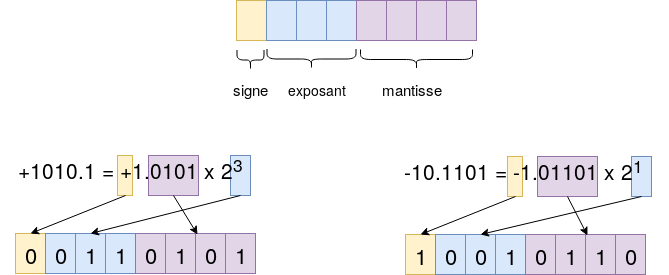
\includegraphics[width=11cm]{img/format_general_flottant.png}
  \end{center}

\end{frame}


  \begin{frame}
	\frametitle{Représentation des nombres flottants}
	\begin{block}{Exercice}
		Quelle est la valeur du nombre représenté en virgule flottante
		de la façon suivante, avec |e|=3 |m|=4 ?  1 110 1001
	\end{block}
	\only<2>{
		\begin{block}{Solution}
			\begin{center}
				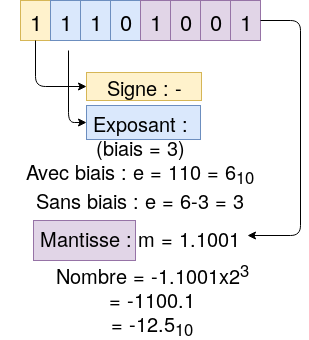
\includegraphics[width=4.2cm]{img/flottant_nombre_a_deviner.png}
			\end{center}
		\end{block}
	}
\end{frame}

\begin{frame}
	\frametitle{Normalisation du codage des flottants}
	
	\begin{block}{Norme IEEE 754 (standard)}
		\begin{itemize}
			\item Format simple précision: 32 bits
			\begin{itemize}
				\item Bit du signe (1~bit);
				\item Exposant (8~bits);
				\item Mantisse (23~bits).
			\end{itemize}
			
			\item Format double précision: 64 bits
			\begin{itemize}
				\item Bit du signe (1~bit);
				\item Exposant (11~bits);
				\item Mantisse (52~bits).
			\end{itemize}
			
			\item Autres formats:
			\begin{itemize}
				\item Simple précision étendue ($\geq{}43$~bits, obsolète);
				\item Double précision étendue ($\geq{}79$~bits, long double de C).
			\end{itemize}
		\end{itemize}
	\end{block}
\end{frame}





\begin{frame}
\frametitle{Problèmes de représentation de certains nombres}

\begin{block}{Comment représenter le 0 ?}
  \begin{itemize}
  \item Avec la notation normalisée (mantisse : \colorbox{red}{1}.bbb x $2^e$), le 0
    est impossible à représenter
  \item Convention : tous les bits à 0 (Ex : 0 000 0000)
  \end{itemize}
\end{block}

\begin{block}{Comment représenter le 1 ?}
  \begin{itemize}
  \item 1 = 1.0 x $2^0$ (mantisse = 0 et exposant = 0)
  \item On le représente comme le 0 alors ?
  \item Non, mantisse = 0 et exposant décalé (pourquoi décalé ?  voir
    exposants négatifs)
  \end{itemize}
\end{block}

\end{frame}

\begin{frame}
\frametitle{Problèmes de représentation de certains nombres}
  \only<1>{
  \begin{block}{Comment représenter les exposants négatifs ?}
    \begin{itemize}
    \item En complément à 2 ?
    \item Non. Pourquoi ? Comparaison des flottants difficile
%    \item Représenter l'exposant avec un décalage (``Biais'')
%    \item Biais = $2^{|e|-1}-1$ (|e| : taille de l'exposant)
%    \item Pour un exposant sur |e| bits : au lieu de représenter les
%      nombres de 0 à $2^{|e|}-1$ (Ex : |e|=8, [0,255]), on 
%      représentera les nombres [-$2^{|e|-1}$-1 , $2^{|e|-1}$] (pour |e|=8,
%      biais = $2^{8-1}$-1 = 127 $\rightarrow$ [-127,128])
    \end{itemize}
  \end{block}
}
  \only<2>{
  \begin{block}{Comment représenter les exposants négatifs ?}
    \begin{itemize}
    \item Encodage : on ajoute le biais\\
       Ex sur 3 bits (biais = 3) : exposant = $2_{10}$ 
      $\rightarrow$ 2+3 = 5 = $101_2$
    \item décodage : on retire le biais\\
      Ex sur 3 bits : $010_2$ $\rightarrow$ 2-3 = -1
    \item Les exposants spéciaux  : (valeurs extrêmes)\\
      Ex : pour |e|=8
      \begin{enumerate}
      \item -127 (0 sans biais) est réservé pour le 0 et les
        nombres ``dénormalisés''
      \item 128 (255 sans biais) est réservé pour les infinis et
        NaN
        \end{enumerate}
    \end{itemize}
  \end{block}
}
  \only<3>{
    \begin{block}{Exercice}
      Écrire le nombre +1 avec un exposant de 3 bits et une mantisse de
      4 bits
    \end{block}
    }

      \only<4>{
    \begin{block}{Solution}
  \begin{center}
    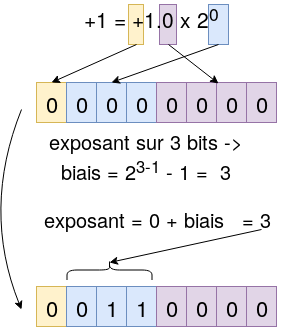
\includegraphics[width=5cm]{img/flottant_nombre_1.png}
  \end{center}

    \end{block}
    }
  \end{frame}
  


% \begin{frame}
% \frametitle{Format d'un nombre en virgule flottante}

% \begin{block}{Format général}
% \begin{center}
% \begin{tabular}{|c|c|c|}
% \hline
% Signe & Exposant décalé & Mantisse\\
% \hline
% 1~bit & $e$~bits & $m$~bits\\
% \hline
% \end{tabular}
% \end{center}
% \end{block}  

% \begin{block}{Décalage de l'exposant}
% \begin{itemize}
% \item Exposants positifs ou négatifs;
% \item Pour les négatifs, pas de complément à~2;
% \item Utilisation d'un décalage: un biais;
% \item Biais = $2^{e-1}-1$;
% \item En simple précision: 127;
% \item En double précision: 1023.
% \end{itemize}
% \end{block}  
% \end{frame}

\begin{frame}
\frametitle{Format d'un nombre en virgule flottante}

\begin{block}{Différents cas}
\begin{center}
\begin{tabular}{|c|c|c|}
  \hline
  Type & Exposant décalé & Mantisse\\
  \hline
  Zéro(s) & 0 & 0\\
  \hline
  Infinis & $2^{|e|}-1$ (que des~1) & 0\\
  \hline
  NaN & $2^{|e|}-1$ (que des~1) & différente de 0\\
  \hline
  Nombres dénormalisés & 0 & différente de 0\\
  \hline
  Nombres normalisés & 1 à $2^{|e|}-2$ & quelconque\\
  \hline
\end{tabular}
\end{center}
\end{block}  
\end{frame}

\begin{frame}
\frametitle{Format d'un nombre en virgule flottante}

\begin{block}{Nombres normalisés}
\begin{itemize}
\item $n=s\times{}m\times{}2^{e}$ (valeur décimale du nombre réel);
\item $s$ = $\pm{}1$ (+1 si bit de signe à 0, -1 sinon);
\item $e$ = exposant décalé ($e_d$) - biais;
\item $m$ = 1 + mantisse ($1\leq{}m<2$).
\end{itemize}
\end{block}

\begin{block}{Nombres dénormalisés (nombres avec valeur très proche de 0)}
\begin{itemize}
\item $n=s\times{}m\times{}2^{e}$ (valeur décimale du nombre réel);
\item $s$ = $\pm{}1$ (+1 si bit de signe à 0, -1 sinon);
\item $e$ = $(-2^{|e|-1}+1)+1$ = $-2^{|e|-1}+2$;
\item $m$ = 0 + mantisse ($0<m<1$).
\end{itemize}
\end{block}
\end{frame}

\begin{frame}
  \frametitle{Nombres positifs représentables sur 8 bits
    (|e|=4)}
  \vspace{-1cm}
\hspace{-1cm}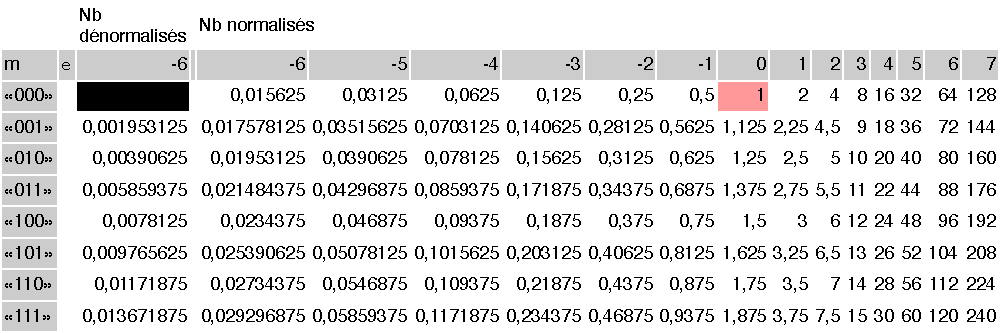
\includegraphics[width=11.5cm]{img/flottants_sur_8_bits.pdf}

\end{frame}
  
\begin{frame}
\frametitle{Exemples de nombres dénormalisés en simple précision}
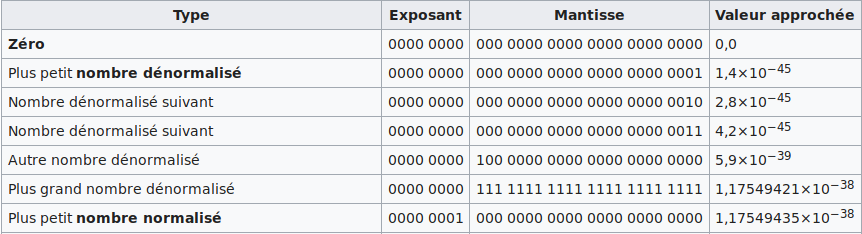
\includegraphics[width=11.5cm]{img/simple_precision_denorm.png}

\end{frame}

\begin{frame}
\frametitle{Exemples de nombres normalisés en simple précision}
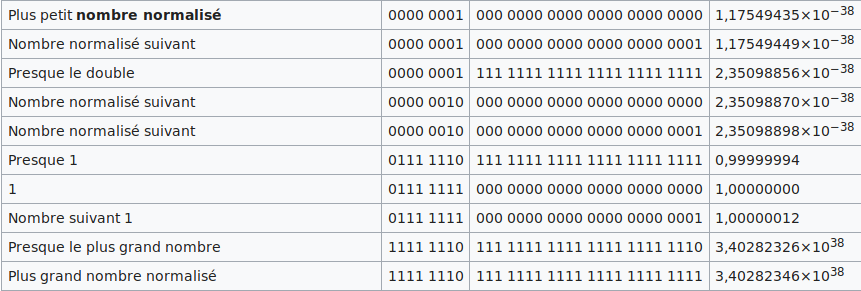
\includegraphics[width=11.5cm]{img/simple_precision.png}

\end{frame}


\begin{frame}
\frametitle{D'une représentation à l'autre}

\begin{block}{Exemples en simple précision}
\begin{itemize}
\item Valeur décimale de:\\
\begin{center}
  0 10000010 11000000000000000000000
  \end{center}
\begin{itemize}
\item 0 = positif $\Rightarrow$ s=+1;
\item $e_d$ = $10000010_2$ = 130$_{10}$, e = 130$_{10}$ - 127$_{10}$ =
  $3_{10}$;
\item m = 1.11$_2$ = 1.75$_{10}$;
\item n = $+1 \times{}  1.75\times{}2^3=14$;
  \item ou bien n = $+1 \times{} 1.11_2\times{}2^3=1110_2=14$.
\end{itemize}
\end{itemize}
\end{block}
\end{frame}

\begin{frame}
\frametitle{D'une représentation à l'autre}

\begin{block}{Exemples en simple précision}
\begin{itemize}
\item Valeur binaire de : -$118.625_{10}$
\begin{itemize}
\item bit de signe = 1 (négatif);
\item $118_{10}$ = 1110110$_2$;
\item $0.625\times{}2=1.25=\underline{1}+0.25$;
\item $0.25\times{}2=0.5=\underline{0}+0.5$;
\item $0.5\times{}2=1.0=\underline{1}+0$;
\item 0.625 = 101$_2$;
\item $118.625_{10}$ = 1110110.101$_2$ = $1.110110101\times{}2^6$;
\item $e_d$ = 6 + 127 = 133 = 10000101$_2$;
\item représentation : 1 10000101 11011010100000000000000.
\end{itemize}
\end{itemize}
\end{block}
\end{frame}

\begin{frame}
\frametitle{D'une représentation à l'autre}

\begin{block}{Exercice en simple précision}
\begin{itemize}
\item Donner la valeur décimale de:
\begin{itemize}
\item 1 10000010 11110110000000000000000.
\end{itemize}

\item Donner la représentation de:
\begin{itemize}
\item 3.1416015625$_{10}$.
\end{itemize}

\item Que se passe-t-il si l'on souhaite représenter 3.14$_{10}$?

\item Comment obtient-on le plus petit nombre normalisé positif?

\item Comment obtient-on le plus petit nombre dénormalisé positif?
\end{itemize}
\end{block}
\end{frame}

\begin{frame}
\frametitle{D'une représentation à l'autre}
\vspace{-1.2cm}
\begin{block}{Correction}
\begin{itemize}
\item Donner la valeur décimale de:
\begin{itemize}
\item 1 10000010 11110110000000000000000;
\item Solution: -15.6875.
\end{itemize}

\item Donner la représentation de:
\begin{itemize}
\item 3.1416015625$_{10}$;
\item Solution: 0 10000000 10010010001000000000000.
\end{itemize}

\item Pour 3.14$_{10}$, il n'est pas exactement représentable. Il est donc
approximé (on s'arrête à la fin de la mantisse, troncature).

\item Plus petit nombre normalisé positif:
\begin{itemize}
\item Plus petit $e_d$ non nul (00000001) et mantisse nulle;
\item Résultat: $2^{-126}$.
\end{itemize}    

\item Plus petit nombre dénormalisé positif:
\begin{itemize}
\item Exposant décalé: 0 (par définition);
\item Mantisse: 00000000000000000000001;
\item Résultat: $2^{-23}\times{}2^{-126}=2^{-149}$.
\end{itemize}
\end{itemize}
\end{block}
\end{frame}

\begin{frame}
\frametitle{Calculs sur les flottants}

\begin{block}{Addition}
\begin{itemize}
\item Addition de:
\begin{itemize}
\item X = 0 10000001 11000000000000000000000;
\item Y = 0 01111111 00000000000000000000000;
\item X = $1.11\times{}2^2$, Y = $1.0\times{}2^0$;
\item On aligne les exposants (sur le plus grand);
\item Y = $0.01\times{}2^2$;
\item On additionne les mantisses:\\
1.11000000000000000000000 +\\
0.01000000000000000000000 =\\
10.00000000000000000000000
\item Résultat = $10.0\times{}2^2$ = $1.0\times{}2^3$;
\item Codage : 0 10000010 00000000000000000000000.
\end{itemize}
\end{itemize}
\end{block}
\end{frame}

\begin{frame}
\frametitle{Calculs sur les flottants}

\begin{block}{Exercice}
\begin{itemize}
\item Additionner les deux flottants suivants:
\begin{itemize}
\item X = 0 10000001 11000000000000000000000;
\item Y = 0 01111110 11000000000000000000011.
\end{itemize}

\item Additionner les deux flottants suivants:
\begin{itemize}
\item X = 0 11111110 11000000000000000000000;
\item Y = 0 01111111 11000000000000000000000.
\end{itemize}
\end{itemize}
\end{block}
\end{frame}

\begin{frame}
\frametitle{Calculs sur les flottants}

\begin{block}{Solution : Additionner les deux flottants}
\begin{itemize}
\item X = 0 10000001 11000000000000000000000;
\item Valeur de X :
  \begin{itemize}
  \item $e_d$ = 10000001$_2$ = 129$_{10}$, e = 129-127 = 2
  \item Valeur de X = 1.11 x 2$^2$
  \end{itemize}
  
\item Y = 0 01111110 11000000000000000000011.
  \item Valeur de Y :
  \begin{itemize}
  \item $e_d$ = 01111110$_2$ = 126$_{10}$, e = 126-127 = -1
  \item Valeur de Y = 1.11000000000000000000011 x 2$^{-1}$
  \end{itemize}
\item Aligner les exposants :\\ Valeur de Y = 0.00111 x 2$^2$
  \textbf{(perte de précision)}
\item Somme = 1.11111 x 2$^2$
\item Codage : 0~~10000001~~11111000...0
\end{itemize}
\end{block}
\end{frame}

\begin{frame}
\frametitle{Calculs sur les flottants}

\begin{block}{Solution : Additionner les deux flottants}
\begin{itemize}
\item X = 0 11111110 11000000000000000000000
\item Valeur de X :
  \begin{itemize}
  \item $e_d$ = 11111110$_2$ = 254$_{10}$, e = 254-127 = 127
  \item Valeur de X = 1.11 x 2$^{127}$ (Très grand nombre)
  \end{itemize}
  
\item Y = 0 01111111 11000000000000000000000
  \item Valeur de Y :
  \begin{itemize}
  \item $e_d$ = 01111111$_2$ = 127$_{10}$, e = 127-127 = 0
  \item Valeur de Y = 1.11 x 2$^{0}$
  \end{itemize}
\item Aligner les exposants :\\ Valeur de Y = 0.00....0 x 2$^{127}$
  \textbf{(perte de précision)}
\item Somme = 1.11 x 2$^{127}$ = Valeur de Y (absorption)
\item Codage = X
\end{itemize}
\end{block}
\end{frame}

\begin{frame}
\frametitle{Calculs sur les flottants}

\begin{block}{Exercice}
\begin{itemize}
\item Multiplier les deux flottants suivants:
\begin{itemize}
\item X = 0 10000001 01000000000000000000000;
\item Y = 0 01111111 11000000000000000000000.
\end{itemize}
\end{itemize}
\end{block}
\end{frame}

\begin{frame}
\frametitle{Calculs sur les flottants}

\begin{block}{Correction}
\begin{itemize}
\item Multiplier les deux flottants suivants:
\begin{itemize}
\item X = 0 10000001 01000000000000000000000;
\item Y = 0 01111111 11000000000000000000000;
\item X = $1.01\times{}2^2$, Y = $1.11\times{}2^0$;
\item Addition des exposants: $2+0=2$;
\item Multiplication des mantisses: $1.01\times{}1.11=10.0011$;
\item Résultat = $1.00011\times{}2^3$ (exposant incrémenté);
\item Codage: 0 10000010 00011000000000000000000.
\end{itemize}
\end{itemize}
\end{block}
\end{frame}

\begin{frame}
\frametitle{Diapos et références}

\begin{block}{Diapos constuites sur la base du cours de :}
  David Delahaye, professeur à la FDS (mon prédécesseur)
\end{block}

\begin{block}{Références bibliographiques}
\begin{itemize}
\item Paolo Zanella, Yves Ligier et Emmanuel Lazard. Architecture et
  technologie des ordinateurs - 6e éd. - Cours et exercices
  corrigés. Septembre 2018
\item Utilisation des nombres à virgule flottante (risques) :\\
  \footnotesize
  \url{https://www.ekito.fr/people/les-nombres-virgule-flottante/}
  \normalsize
\end{itemize}
\end{block}

\end{frame}

\end{document}
